\documentclass[11pt, oneside]{article} 
\usepackage{mathptmx}
\usepackage{amsmath, amsthm, amssymb, calrsfs, wasysym, verbatim, bbm, color, graphics, geometry}
\usepackage{graphicx}
\usepackage{float}
\usepackage{longtable}
\usepackage{rotating}
\usepackage{adjustbox}
\usepackage{booktabs}
\usepackage{caption}
\usepackage[english]{babel}
\usepackage[utf8]{inputenc}
\usepackage[table]{xcolor}
\usepackage{multicol}
\usepackage{hyperref}
\usepackage{amsmath}

\geometry{tmargin=.75in, bmargin=.75in, lmargin=.75in, rmargin = .75in}  

\newcommand{\R}{\mathbb{R}}
\newcommand{\C}{\mathbb{C}}
\newcommand{\Z}{\mathbb{Z}}
\newcommand{\N}{\mathbb{N}}
\newcommand{\Q}{\mathbb{Q}}
\newcommand{\Cdot}{\boldsymbol{\cdot}}

\newtheorem{thm}{Theorem}
\newtheorem{defn}{Definition}
\newtheorem{conv}{Convention}
\newtheorem{rem}{Remark}
\newtheorem{lem}{Lemma}
\newtheorem{cor}{Corollary}

\font\arial=cmr12 at 40pt
\title{{\arial AN2DL Second Homework}}
\font\calibri=cmr12 at 20pt
\author{{\calibri Mauro Famà,   Sofia Martellozzo,   Lorenzo Mondo\\ \\
        Group cANNoli}}
\date{Academic Year 2022-2023}

\begin{document}

\maketitle
\begin{center}
    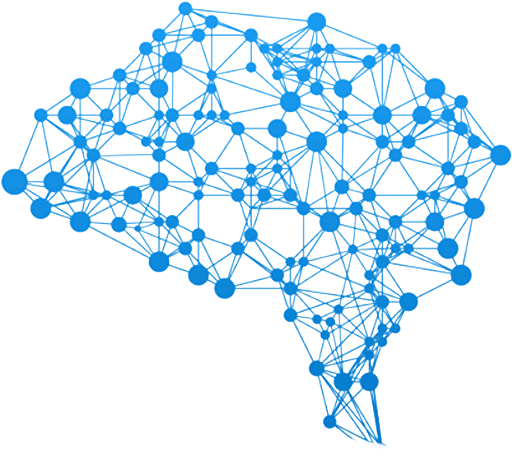
\includegraphics[scale=0.43]{images/title.png}
\end{center}
\newpage
\vspace{.25in}

%---------------------------------------%

\section{Introduction}
This report describes a multivariate time series classification project in which several artificial neural network models were used. The obtained results were compared and analysed to identify the most performant model for this type of problem.\\The dataset provided for this project consists of multivariate time series with 6 variables and a total of 12 classes: "Wish," "Another," "Comfortably," "Money," "Breathe," "Time," "Brain," "Echoes," "Wearing," "Sorrow," "Hey," and "Shine." The dataset is heavily imbalanced: the class with the most samples is "Sorrow" with 777 samples, while the class with the fewest samples is "Wish" with 34 samples.\\In the next chapters is provided an overview of the techniques used, the different models implemented and a detailed description of the results obtained. In addition, some concluding thoughts are presented on the advantages and disadvantages of the different models and on the factors that influence their performance.

%---------------------------------------%
\section{Techniques}
\subsection{Data Augmentation}
Data augmentation attempts to fix class imbalance by generating extra patterns in the minority classes. While data augmentation is a common practice in image recognition with neural networks, it is not established as a standard procedure for time series recognition.\\ 
Similar to data augmentation for images, most data augmentation techniques for time series are based on random transformations of the training data. For example, adding random noise (jittering) , slicing or cropping , scaling, random warping in the time dimension, and frequency warping. The problem with random transformation-based data augmentation is that there is a diverse amount of time series, each having different properties, and not every transformation is applicable to every dataset. For this reason with the new samples generated with these techniques no improvement has been achieved by our models, so we decide to use another augmentation model, called SMOTE.\\  
\textbf{SMOTE} first selects a minority class instance $a$ randomly and finds its $k$ nearest minority class neighbors. The synthetic instance is then created by choosing one of the $k$ nearest neighbors $b$ at random and connecting $a$ and $b$ to form a line segment in the feature space. The synthetic instances are generated as a convex combination of the two chosen instances $a$ and $b$. With this technique we achieved significantly better results.

\subsection{Pre-processing}
Normalization and standardization are two techniques used to prepare data for analysis. Both techniques are used to standardize the values of variables in order to make them comparable to each other, but they differ in how they are performed.
\subsubsection{Normalization}
Normalization consists of transforming the values of each variable into a specific range, usually between 0 and 1. One way to perform normalization is through min-max normalization, which scales the values of each variable between a minimum and maximum value. The formula for min-max normalization is as follows:
\[ x_{norm} = \frac{x - x_{min}}{x_{max} - x_{min}} \]\
where x is the value to be normalized, $x_{min}$ is the minimum value of the variable, $x_{max}$ is the maximum value of the variable, and $x_{norm}$ is the normalized value.
Normalization is often used when it is important to maintain the original range of values or when you want to avoid privileging some variables over others.
\subsubsection{Standardization}
Standardization, on the other hand, consists of transforming the values of each variable into a standard scale, where the mean is 0 and the standard deviation is 1. Standardization is performed using the following formula:
\[x_{std} = \frac{x - \mu}{\sigma} \]
where x is the value to be standardized, $\mu$ is the mean of the variable, $\sigma$ is the standard deviation of the variable, and $x_{std}$ is the standardized value.
Standardization is often used when it is important to standardize values on a standard scale or when you want to avoid variables with high values from having too much influence on the analysis.\\\\
In our case, model training performed better using standardization instead of normalization for several reasons. First, standardization is more suited to our data as the values of the variables have a normal distribution. In addition, standardization allows us to avoid privileging some variables over others, as all variables are standardized on the same scale. Finally, standardization enables us to use all the information available in our data, as normalization does not limit variables' values to a specific range.

%---------------------------------------%
\section{Development Models}
In our experiments, we split the dataset into train and validation sets using an 80/20 split, maintaining the proportion of time series for each class in both sets. We used the train set to train the models and the validation set to evaluate their performance.\\
In some cases, we trained the models without any preprocessing of the data. In other cases, we applied pre-processing techniques such as normalization, standardization or data augmentation to the data before training the models.
\subsection{LSTM (Long Short-Term Memory)}
A particular type of artificial neural network that succeeds in processing sequential data is the LSTM. In addition to having input and output gates, LSTM cells also have a cell state. While the cell state enables the LSTM to retain significant information for extended periods of time, the input and output gates regulate the flow of information into and out of the cell. In order to recall pertinent information from earlier in the sequence and utilize it to forecast future events, LSTMs can leverage their cell state when processing sequential data. This makes LSTMs particularly useful for tasks like multivariate time series classification, where long-term dependencies between elements in the time series are important.\\
For this multivariate time series classification problem, we combined a convolutional neural network with a Long Short-Term Memory (LSTM) neural network.\\\\
We trained this model using pre-processed input with the data augmentation technique described in Section 2.1, obtaining an accuracy of 0.6809\% in the final phase of the competition.
\subsection{BiLSTM (Bidirectional Long Short-Term Memory)}
BiLSTM is a variant of LSTM that processes sequential data in both forward and backward directions. This allows BiLSTM to capture dependencies between elements in the sequence both forwards and backward, which can be especially useful for tasks like multivariate time series classification where both long-term and short-term dependencies are important. In a BiLSTM model, the input data is processed by two separate LSTM networks, one that processes the data from the beginning to the end of the sequence and one that processes the data from the end to the beginning. The outputs of these two networks are then combined to produce a final prediction or classification.\\
In our experiments we played around with several BiLSTM model setups, varying the amount of neurons in the layers and using preprocessing and data augmentation methods.\\\\
The BiLSTM model setup, composed of two BiLSTM layers and 128 neurons in each layers, achieved an accuracy of 66\% without any pre-processing and 68\% with data augmentation.

\subsection{1D Convolutional Neural Networks (CNNs)}
1D Convolutional Neural Networks are a type of artificial neural network that is particularly effective at extracting features from sequential data. CNNs use convolutional filters to learn patterns in the data and use those patterns to make predictions or decisions. In a 1D CNN, the filters are applied to the input data along the time dimension, allowing the model to learn temporal patterns in the data. This makes 1D CNNs well-suited for tasks like multivariate time series classification, where the relationships between different time series are important for making accurate predictions.\\\\
The 1D CNN model that we used in our experiments consists of a series of convolutional layers that apply a convolution operation to the input data, as well as pooling layers that down-sample the data by taking the maximum value in a window of time steps. The model also includes a global average pooling layer, which averages the values of the output of the convolutional layers across the time dimension, and a dropout layer, which randomly drops out a fraction of the input units to prevent overfitting. The model also includes two fully-connected layers that apply an activation function to the input data. The output of the model is a fully-connected layer with a softmax activation function, which produces a probability distribution over the possible classes.
\\
We trained several configurations of the 1DCNN model. The configuration that achieved the best performance in terms of accuracy (68.2\%) in the final phase of the competition was designed wih 1024 neurons in the convolutional and dense layers and was trained using data augmentation techniques.

\subsection{VGG}
We also developed various VGG models (11, 13, 16 and 19). The structure, which was built for 2D convolutional layers, had to be modified in order to work with 1D convolutional layers and with the given problem.
For this reason, we did not use the already built Keras models but we designed them entirely from scratch.\\\\
The obtained results were good (around 50-60\% accuracy), but not enough to be compared with the results of the already presented models.
%---------------------------------------%
\section{Final Model - ResNet}
The network uses 1D convolutional layers to extract features from the time series and then uses batch normalization layers and ReLU activation function to improve the model's performance.\\
The network consists of three blocks, each of which consists of three Conv1D layers and a batch normalization layer. Each block also uses a shortcut layer which adds the input of the block to the output of the third Conv1D layer of the block. This allows the network to "skip" directly to the output of the block without going through all of its intermediate layers, which can help reduce the risk of the model's accuracy degrading due to excessive expansion of its depth.
Finally, the network uses a 1D global pooling layer to reduce the size of the extracted features and a densely connected layer to perform the time series classification.
%---------------------------------------%
\section{Conclusions}
In this project, we evaluated the performance of several models for the classification of multivariate time series data.\\
Our results suggest that the ResNet model performed the best in terms of accuracy on the test set, achieving a performance of 68.2\%. The use of data augmentation techniques helped to slightly improve the model's performance. One potential avenue for further improvement could be to generate new time series data using TimeGAN [0], which is a model that uses a generative adversarial network to synthesize time series data.\\\\
In conclusion, our experiments demonstrated that the 1DCNN model is a promising approach for time series classification, and that the use of data augmentation can be helpful in certain cases. However, there is still room for improvement, and further research is needed to identify effective strategies for boosting the accuracy of time series classification models.
%---------------------------------------%
\section*{References}
[0] \href{http://kth.diva-portal.org/smash/get/diva2:1598158/FULLTEXT01.pdf}{Sofia Nord (2021). Multivariate Time Series Data
Generation using Generative
Adversarial Networks
}\\
{[1]} \href{https://journals.plos.org/plosone/article?id=10.1371/journal.pone.0254841}{Brian Kenji Iwana, Seiichi Uchida. An empirical survey of data augmentation for time series classification with neural networks}
\end{document}
